\chapter{Proposed System and Objectives}

\section{Proposed System Overview}%
\label{sec:system_overview}
To demonstrate the efficacy of a source synchronous system we propose a single
pseudorandom binary sequence (PRBS) source that optically transmits over two
channels to a single reciever. If transmission is alternated the effect is that
the reciever would recieve bursts of data from two different channels. If the
full PRBS sequence is recieved then the system would be working correctly.\\ An
overview of the system is shown in Figure~\ref{fig:overview}. 

\begin{figure}[h]
    \centering
    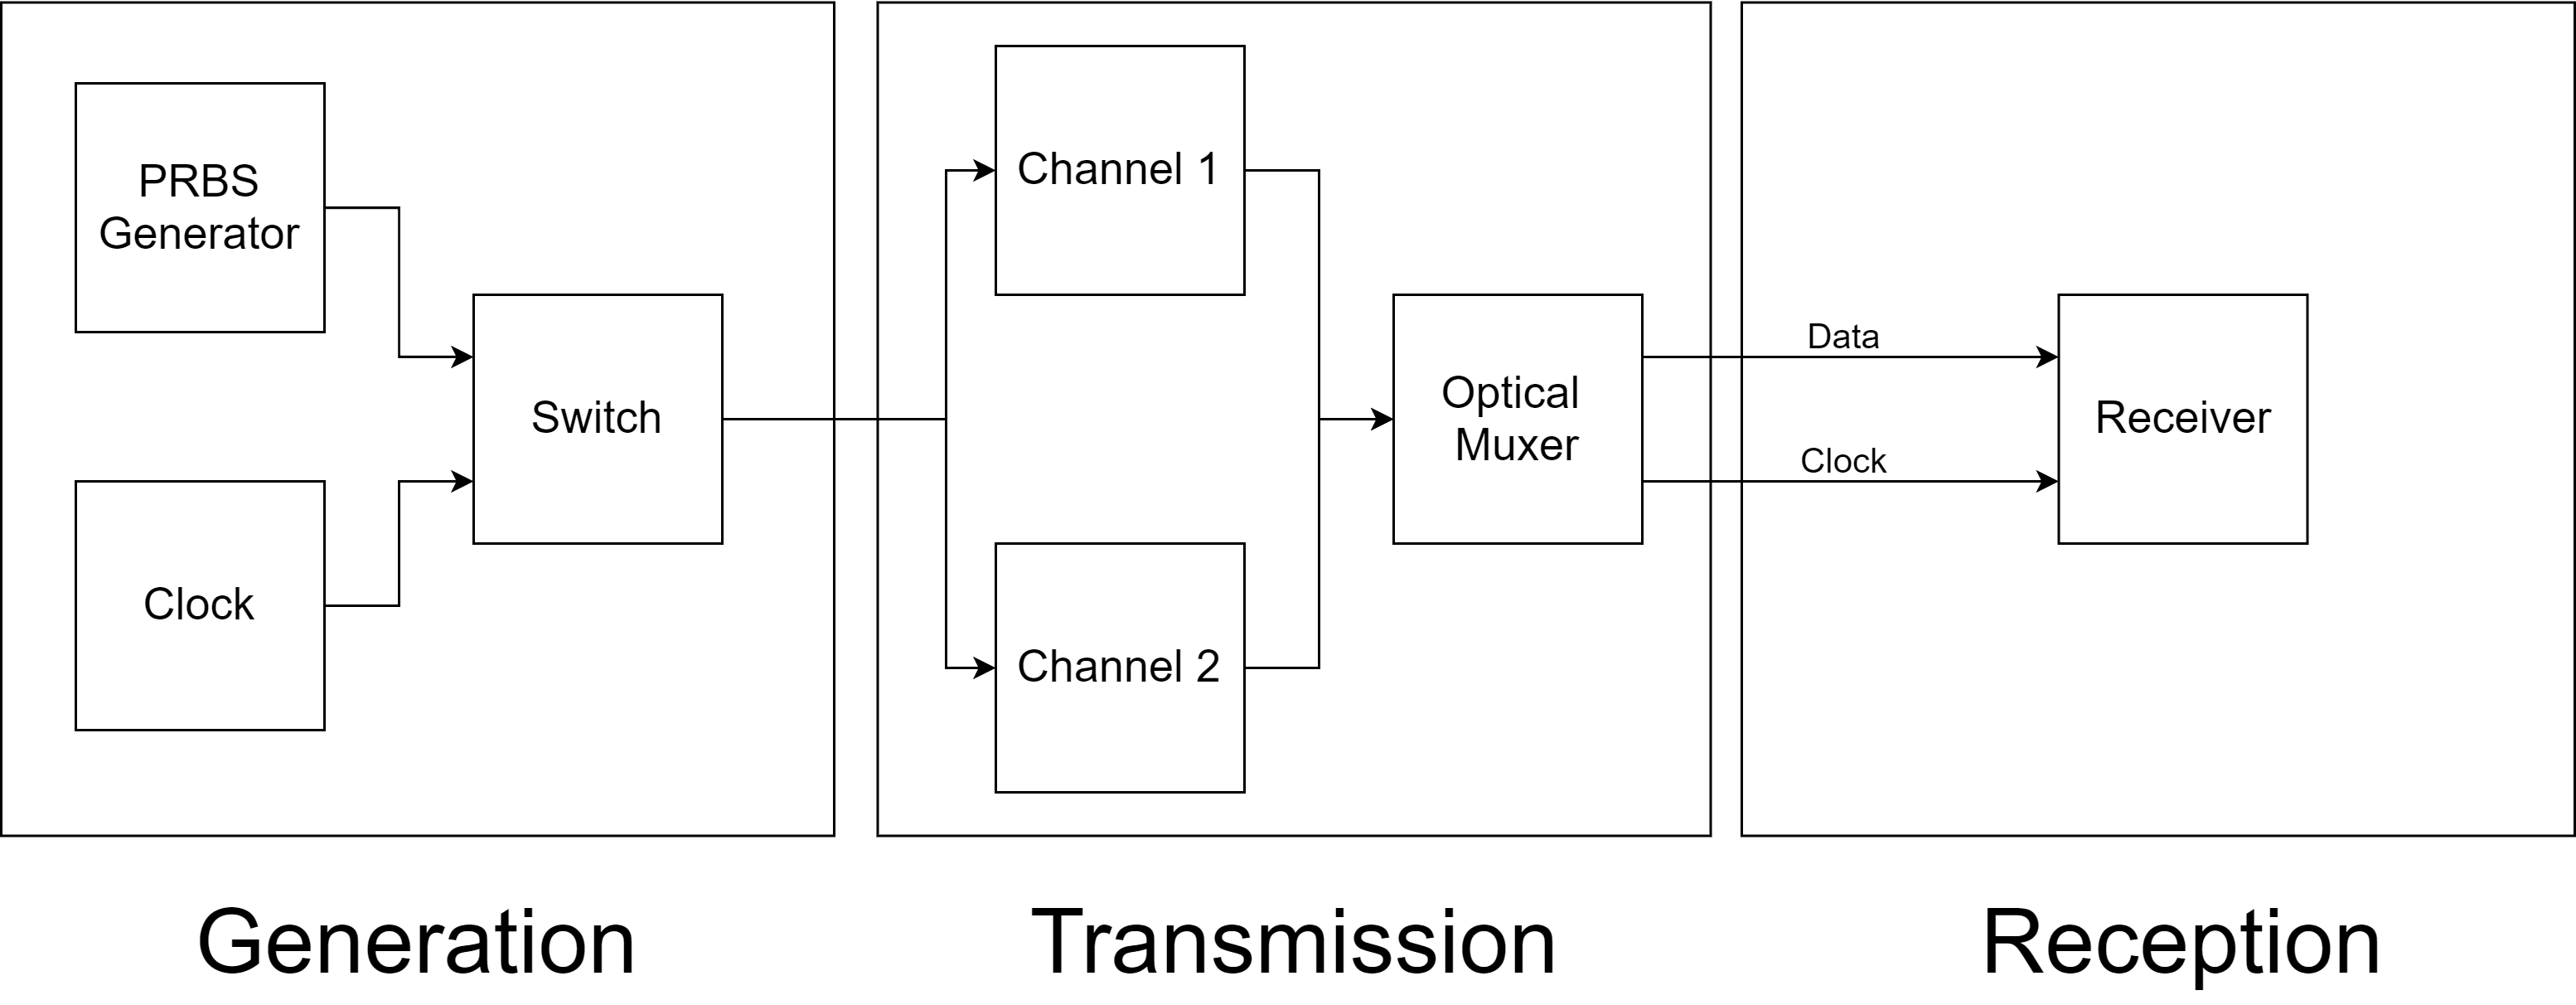
\includegraphics[width=1\linewidth]{img/overview.png}
    \caption{Overview of System}%
    \label{fig:overview}
\end{figure}

\section{Objectives}%
\label{sec:objectives}
The overall objective is to demonstrate successful burst source-synchronous
communication for comparison with a system that uses a CDR.
\noindent
Overall we can break down the project to the following sub-objectives: 
\begin{itemize}
    \item Burst mode PRBS transmission over two channels alongside clock
    \item Transmit data optically and mux the two channels together
    \item Source synchronous reception of PRBS data 
\end{itemize}
